\hypertarget{sph_8cpp}{
\section{sph.cpp File Reference}
\label{sph_8cpp}\index{sph.cpp@{sph.cpp}}
}
{\tt \#include $<$iostream$>$}\par
{\tt \#include $<$fstream$>$}\par
{\tt \#include $<$string$>$}\par
{\tt \#include $<$cstdio$>$}\par
{\tt \#include $<$cstdlib$>$}\par
{\tt \#include $<$ctime$>$}\par
{\tt \#include $<$cmath$>$}\par
{\tt \#include \char`\"{}glbfunc.h\char`\"{}}\par
{\tt \#include \char`\"{}glbcls.h\char`\"{}}\par


Include dependency graph for sph.cpp:\nopagebreak
\begin{figure}[H]
\begin{center}
\leavevmode
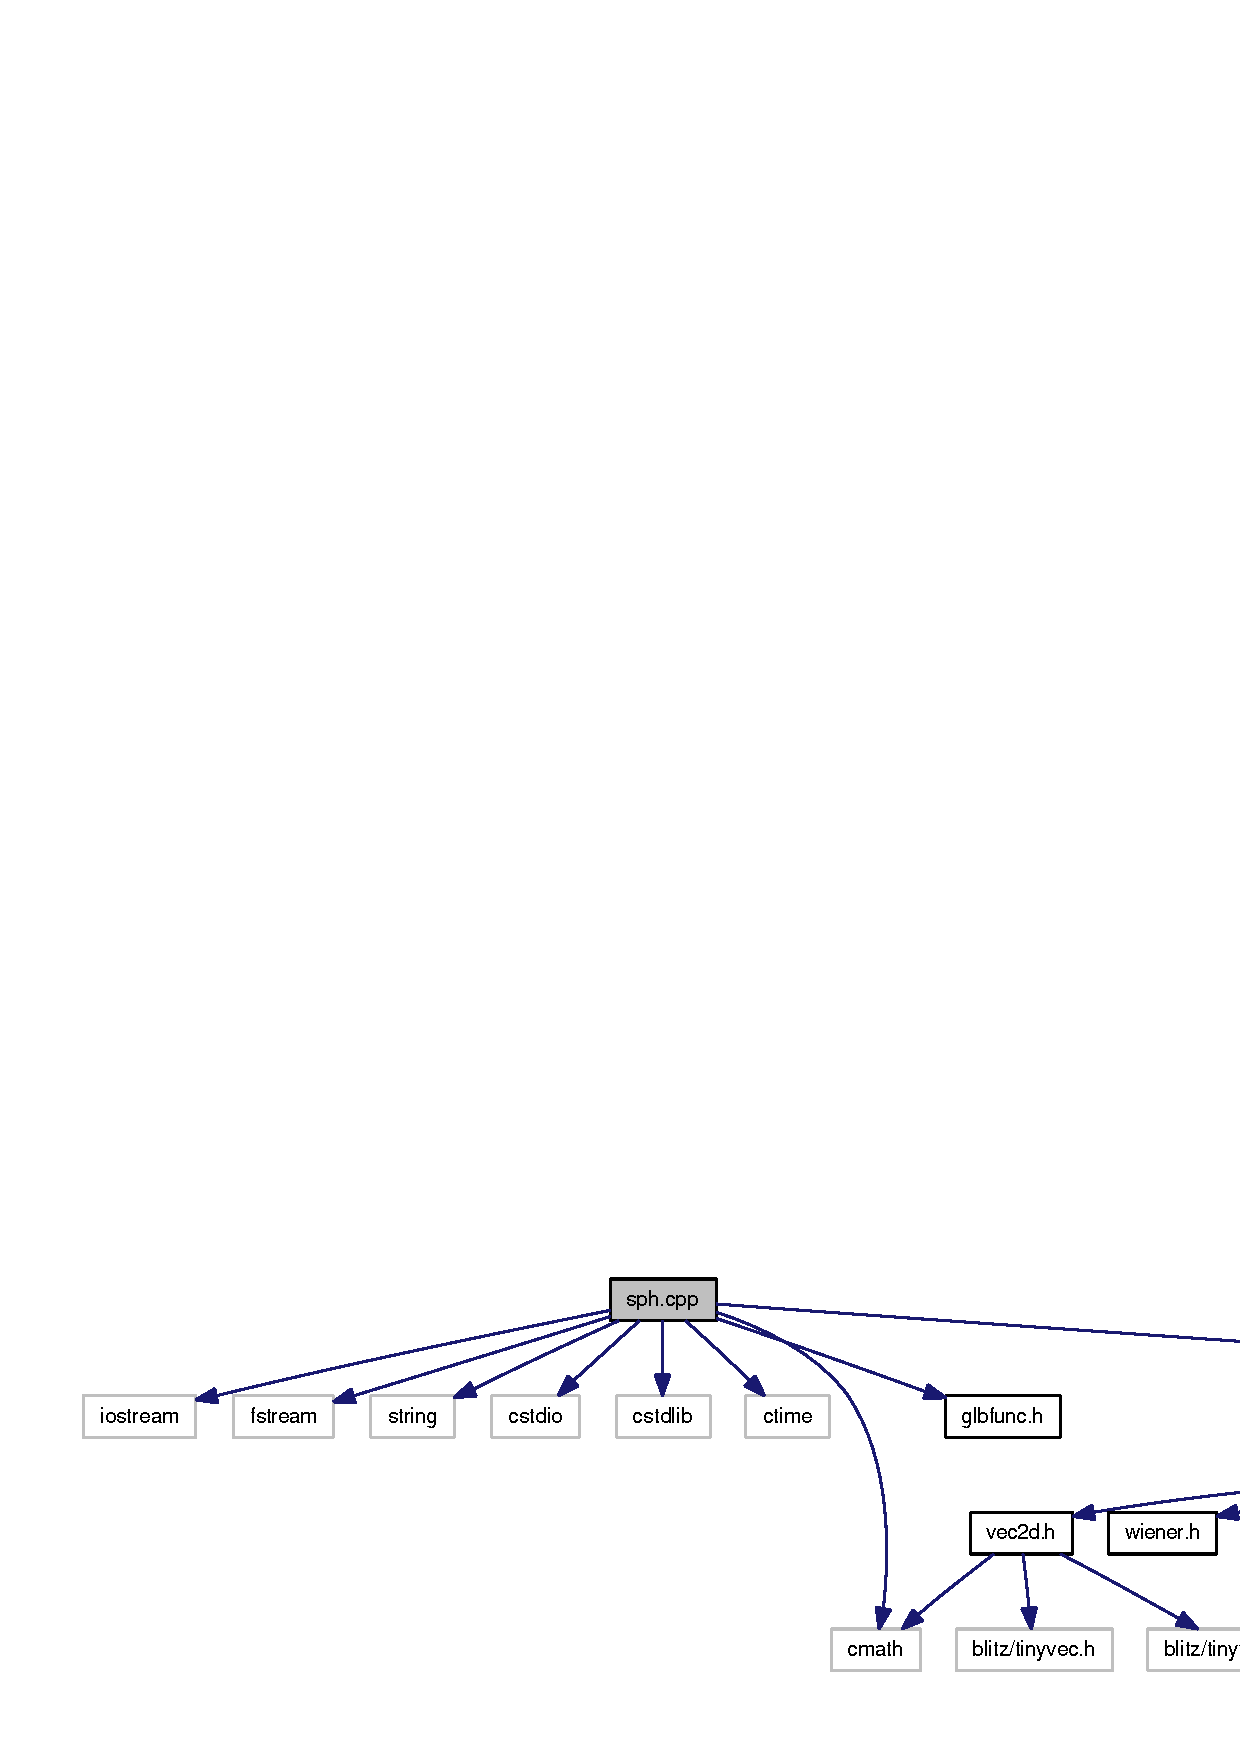
\includegraphics[width=420pt]{sph_8cpp__incl}
\end{center}
\end{figure}
\subsection*{Functions}
\begin{CompactItemize}
\item 
int \hyperlink{sph_8cpp_0ddf1224851353fc92bfbff6f499fa97}{main} (int argc, char $\ast$argv\mbox{[}$\,$\mbox{]})
\begin{CompactList}\small\item\em The main program. \item\end{CompactList}\end{CompactItemize}
\subsection*{Variables}
\begin{CompactItemize}
\item 
\hypertarget{sph_8cpp_a50583a118c0a3e801d3e48a45b6a259}{
double \hyperlink{sph_8cpp_a50583a118c0a3e801d3e48a45b6a259}{k\_\-bltz} = 1.380662e-023}
\label{sph_8cpp_a50583a118c0a3e801d3e48a45b6a259}

\begin{CompactList}\small\item\em Bltzmann constant, will be non-dimensionalized in the program. \item\end{CompactList}\end{CompactItemize}


\label{_details}
\hypertarget{_details}{}
\subsection{Detailed Description}
\begin{Desc}
\item[Author:]Xiangyu Hu $<$\href{mailto:Xiangyu.Hu@aer.mw.tum.de}{\tt Xiangyu.Hu@aer.mw.tum.de}$>$ 

changes by: Martin Bernreuther $<$\href{mailto:Martin.Bernreuther@ipvs.uni-stuttgart.de}{\tt Martin.Bernreuther@ipvs.uni-stuttgart.de}$>$ 

changes by: Andreas Mattes \end{Desc}


\subsection{Function Documentation}
\hypertarget{sph_8cpp_0ddf1224851353fc92bfbff6f499fa97}{
\index{sph.cpp@{sph.cpp}!main@{main}}
\index{main@{main}!sph.cpp@{sph.cpp}}
\subsubsection[{main}]{\setlength{\rightskip}{0pt plus 5cm}int main (int {\em argc}, \/  char $\ast$ {\em argv}\mbox{[}$\,$\mbox{]})}}
\label{sph_8cpp_0ddf1224851353fc92bfbff6f499fa97}


The main program. 

Starts the initialization methods and contains the main computation loop \begin{Desc}
\item[Parameters:]
\begin{description}
\item[{\em argc}]The number of command line arguments, should be two: program name (by default) and project name \item[{\em argv}]The command line arguments array: by default program name at first position (index 0), and then the project( which is specified when calling the program name (e.g. s./sph ../cases/couette) at index 1 \end{description}
\end{Desc}


\par
 {\bf below the rough structure of the main function:}

initializations

\begin{itemize}
\item global initialization (by defining an object of class \hyperlink{classInitiation}{Initiation} (initialization \char`\"{}automatically\char`\"{} done at this moment (from .cfg or .rst file) by constructor method of \hyperlink{classInitiation}{Initiation} class. That is by the way the reason why the initiation::initiation method does not figure in the call grapf of the main function (constructors are not shwon there)\end{itemize}


\begin{itemize}
\item initiate the weight function\end{itemize}


\begin{itemize}
\item initiate the Moving Least Squares approximation\end{itemize}


\begin{itemize}
\item initiate the particle manager\end{itemize}


\begin{itemize}
\item create materials, forces and real particles\end{itemize}


\begin{itemize}
\item initiate boundary conditions and boundary particles\end{itemize}


\begin{itemize}
\item initialize the time solver\end{itemize}


\begin{itemize}
\item initialize output class (should be the last to be initialized)\end{itemize}


\par
 computation loop starts

\begin{itemize}
\item call the time slover (who iterates over one output time interval)\end{itemize}


\begin{itemize}
\item output results after a time interval\par
\par
 \end{itemize}


Here is the call graph for this function:\nopagebreak
\begin{figure}[H]
\begin{center}
\leavevmode
\includegraphics[width=420pt]{sph_8cpp_0ddf1224851353fc92bfbff6f499fa97_cgraph}
\end{center}
\end{figure}
